\documentclass{article}

% Language setting
% Replace `english' with e.g. `spanish' to change the document language
\usepackage[chinese]{babel}
%-- coding: UTF-8 --
\usepackage[UTF8]{ctex}
% Set page size and margins
% Replace `letterpaper' with `a4paper' for UK/EU standard size
\usepackage[letterpaper,top=2cm,bottom=2cm,left=3cm,right=3cm,marginparwidth=1.75cm]{geometry}

% Useful packages
\usepackage{amsmath}
\usepackage{graphicx}
\usepackage[utf8]{inputenc}
\usepackage{cite}

\usepackage{listings}
\usepackage{xcolor}
\lstset{
    numbers=left, 
    numberstyle= \tiny, 
    keywordstyle= \color{ blue!70},
    commentstyle= \color{red!50!green!50!blue!50}, 
    frame=shadowbox, % 阴影效果
    rulesepcolor= \color{ red!20!green!20!blue!20} ,
    escapeinside=``, % 英文分号中可写入中文
    xleftmargin=2em,xrightmargin=2em, aboveskip=1em,
    framexleftmargin=2em
} 
\usepackage[colorlinks=true, allcolors=blue]{hyperref}

\title{第一次作业}
\author{杜汶珂2019201029}

\begin{document}
\maketitle



\section{任务一}
\subsection{要求}
在bsv区块浏览器查询该笔交易,查找到后截图,

\subsection{解答}
见文末截图
\begin{figure}
\centering
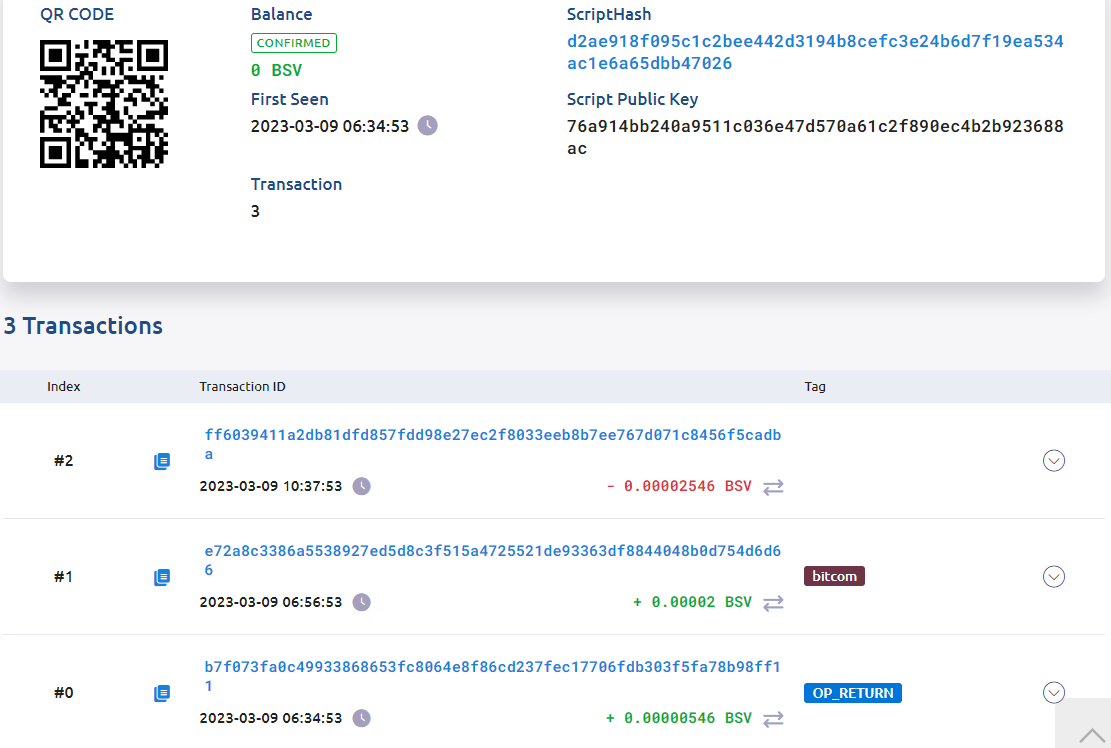
\includegraphics[width=0.8\textwidth,height=0.5\textwidth]{screenshot.png}
\caption{后台截图} \label{fig1}
\end{figure}


\section{任务二}
\subsection{要求}
指出发送地址,接收地址,发送了多少bsv,交易手续费是多少,交易哈希,在哪个高度的区块里
\subsection{解答}
浏览器地址:https://whatsonchain.com/
\par
发送地址:1J4WY4xjmRJxfAspktJpXfhBNuzKZUWAuw
\par
接收地址:1Bo4u2Nno6rr51hsZMu5CDkJaseAM3caQe
\par
发送bsv金额: 0.00002359 BSV
\par
交易手续费:0.00000187
\par
交易哈希:000000000000000008bdf6a887ce1900a90c85e4ee4772de27bd3c34ff79da01
\par
在哪个高度的区块里:782400


\end{document}